\subsection{Extraction of prompt \texorpdfstring{\PsiP}{psi(2S)}/\texorpdfstring{\JPsi}{J/psi} ratio}\label{sec:Charmonia_Analysis_PsiPoverJPsiRatioExtraction}

This section explain the steps followed to measure the ratio of prompt \PsiP over \JPsi meson yields, in \Runpp and \RunPbPb collisions. In this case, due to the low amount of \PsiP mesons present in \RunPbPb collisions, it is not possible to perform a 2D fit to the \mMuMu and \ctau distributions, and an alternative procedure is used instead to measure the prompt charmonium yields.

In order to extract the yields of prompt charmonia, the dimuons are required to pass a \ctau selection that rejects dimuons with \ctau values above a given threshold. The \ctau selection threshold is optimized using simulations as detailed in \sect{sec:Charmonia_Analysis_PsiPYieldExtraction_PromptCut}, keeping 90\% of prompt charmonia while rejecting more than 80\% of nonprompt charmonia. Then, the \PsiP-to-\JPsi yields ratio is extracted from data by fitting the \mMuMu distribution of dimuons passing the \ctau selection, as explained in \sect{sec:Charmonia_Analysis_PsiPYieldExtraction_InvMass}. And finally, the ratio of prompt \PsiP over \JPsi meson yields is determined by subtracting the remaining nonprompt charmonia passing the \ctau selection, as described in \sect{sec:Charmonia_Analysis_PsiPYieldExtraction_NonPromptCorr}.

Due to the more limited \PsiP-meson statistics, the extraction of the ratios of \PsiP over \JPsi meson yields is performed in wider bins compared to the \JPsi-meson analysis. In this case, the fits are performed in two kinematic regions: mid-rapidity ($0 < |\rapMuMu| < 1.6$, $\ptMuMu > 6.5$~\GeVc) and forward rapidity ($1.6 < |\rapMuMu| < 2.4$, $\ptMuMu > 3$~\GeVc). The lower \ptMuMu thresholds in each rapidity region reflects the acceptance of the detector. The measurements are also extracted in different \ptMuMu intervals with boundaries: [6.5, 9, 12, 15, 20, 30]~\GeVc at mid-rapidity and [3, 6.5, 12, 30]~\GeVc at forward rapidity, and in different centrality bins corresponding to: 0-10, 10-20, 20-30, 30-40, 40-50 and 50-100\% at mid-rapidity, and 0-20, 20-40 and 40-100\% at forward rapidity. The analysis bins used in the \PsiP-to-\JPsi double ratio analysis are summarised in \tab{tab:anabins004}.

\subsubsection{Definition of the \ctau selection for prompt charmonia}\label{sec:Charmonia_Analysis_PsiPYieldExtraction_PromptCut}

The threshold of the \ctau selection is tuned using prompt \JPsi simulations, by requiring that the fraction of prompt \JPsi mesons that pass the selection is 90\%, in each analysis bin. The simulated \ctau distributions of prompt and nonprompt signal dimuons in the forward rapidity region, and the corresponding \ctau selection threshold, are shown in \fig{fig:CtauCut}.

\begin{figure}[htb!]
 \centering
 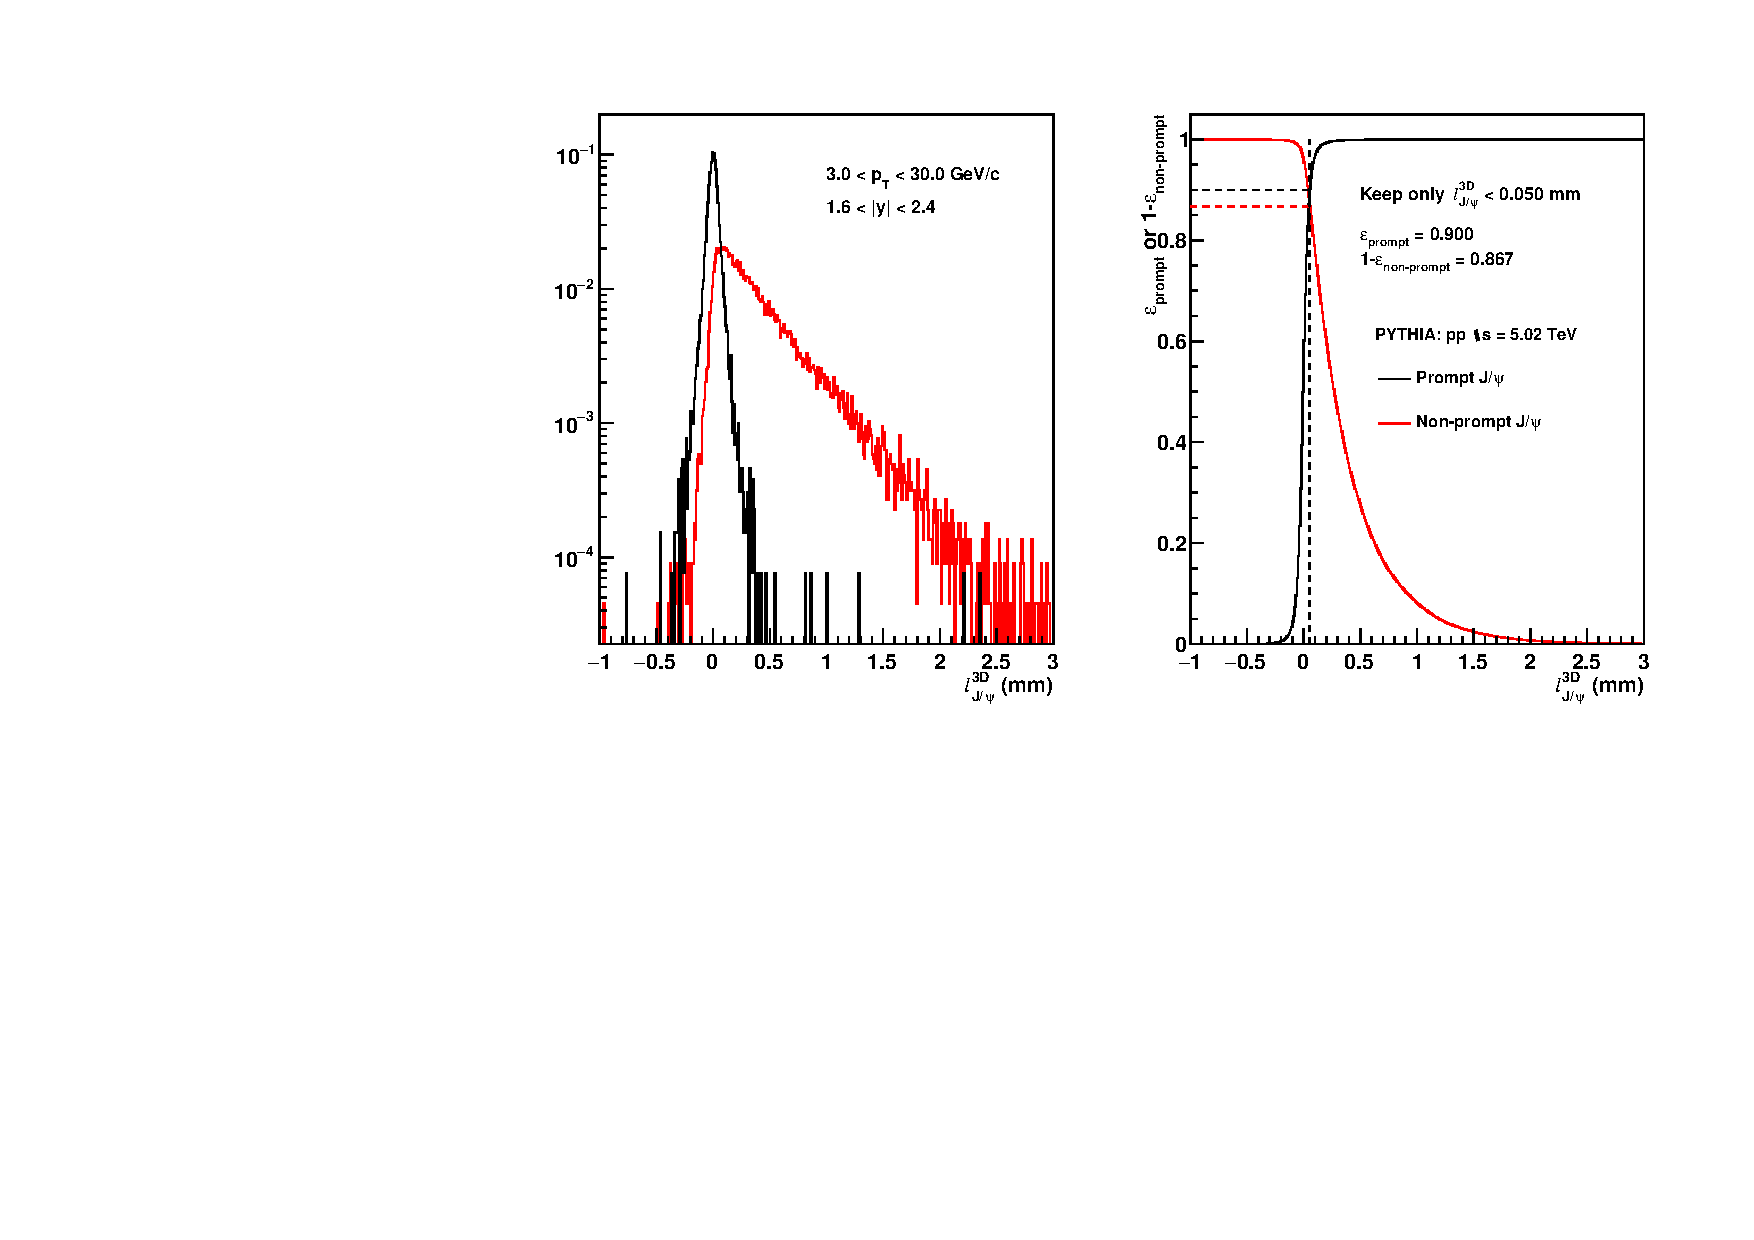
\includegraphics[width=0.85\textwidth]{Figures/Charmonia/Analysis/PsiPSignalExtraction/CtauCut/Jpsi_pp_eff_0p9_Rap_1p6-2p4_Pt_3p0-30p0.pdf}
 \caption{Distribution of \ctau (left) in the \Runpp simulations of prompt and nonprompt \JPsi mesons, and an illustration (right) of the way the \ctau selection threshold is chosen. The results corresponds to the mid-rapidity region $|\rapMuMu| < 1.6$.}
 \label{fig:CtauCut}
\end{figure}

The \ctau selection thresholds extracted from the simulations are found to be consistent between the different collision systems and centrality bins, but they vary between different dimuon \pt and rapidity regions. As a result, the thresholds are extracted in several \ptMuMu regions at mid- and forward rapidity. Then, the profile of the \ctau selection thresholds ($l_{\text{P}}$) with respect of \ptMuMu is fitted separately for each rapidity region, with the following function:

\begin{equation}
 l_{\text{P}}(\ptMuMu) = a + \frac{b}{\ptMuMu}
\end{equation}

where $a$ and $b$ are free parameters. \fig{fig:CtauCutPtDep} displays the fit results of the  $l_{\text{P}}$ profile as a function of \ptMuMu in the two rapidity regions. The \ctau selection, derived from the fits as a function of \ptMuMu, is summarised in:

\begin{linenomath}
  \begin{align}
    \label{eq:CtauPromptCut}
    \ctau < \left\{
      \begin{array}{ll}
        {0.012 + \left(0.23 \big/ \ptMuMu\right)},& \text{if}~{\abs{\rapMuMu} \leq 1.6}\\[0.5cm]
        {0.014 + \left(0.28 \big/ \ptMuMu\right)},& \text{if}~{\abs{\rapMuMu} > 1.6}
      \end{array}\right.
  \end{align}
  \label{eq:CtauCutSel}
\end{linenomath}

\begin{figure}[htb!]
 \centering
 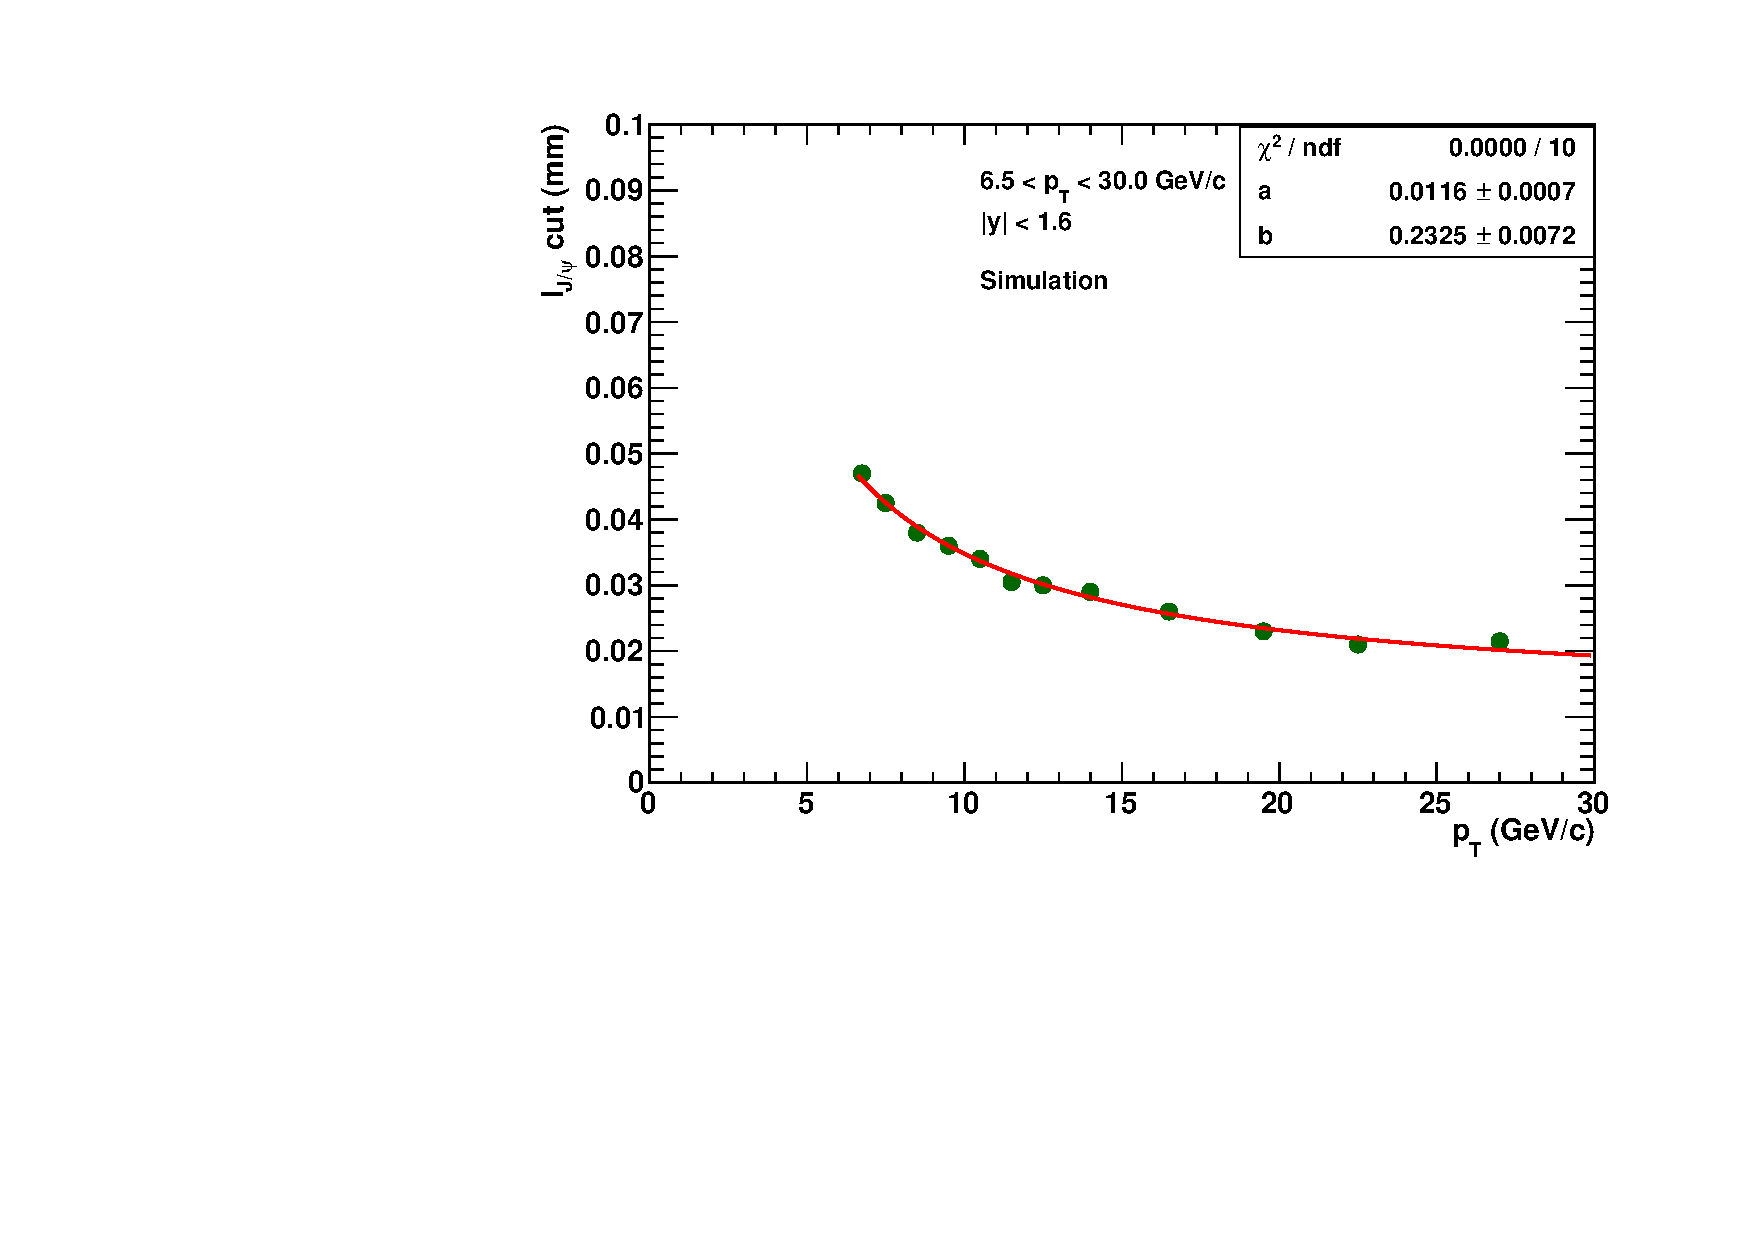
\includegraphics[width=0.48\textwidth]{Figures/Charmonia/Analysis/PsiPSignalExtraction/CtauCut/Jpsi_ppPbPbGlb_eff_0p9_Rap_0p0-1p6_Pt_6p5-30p0_Cent_0-100.pdf}
 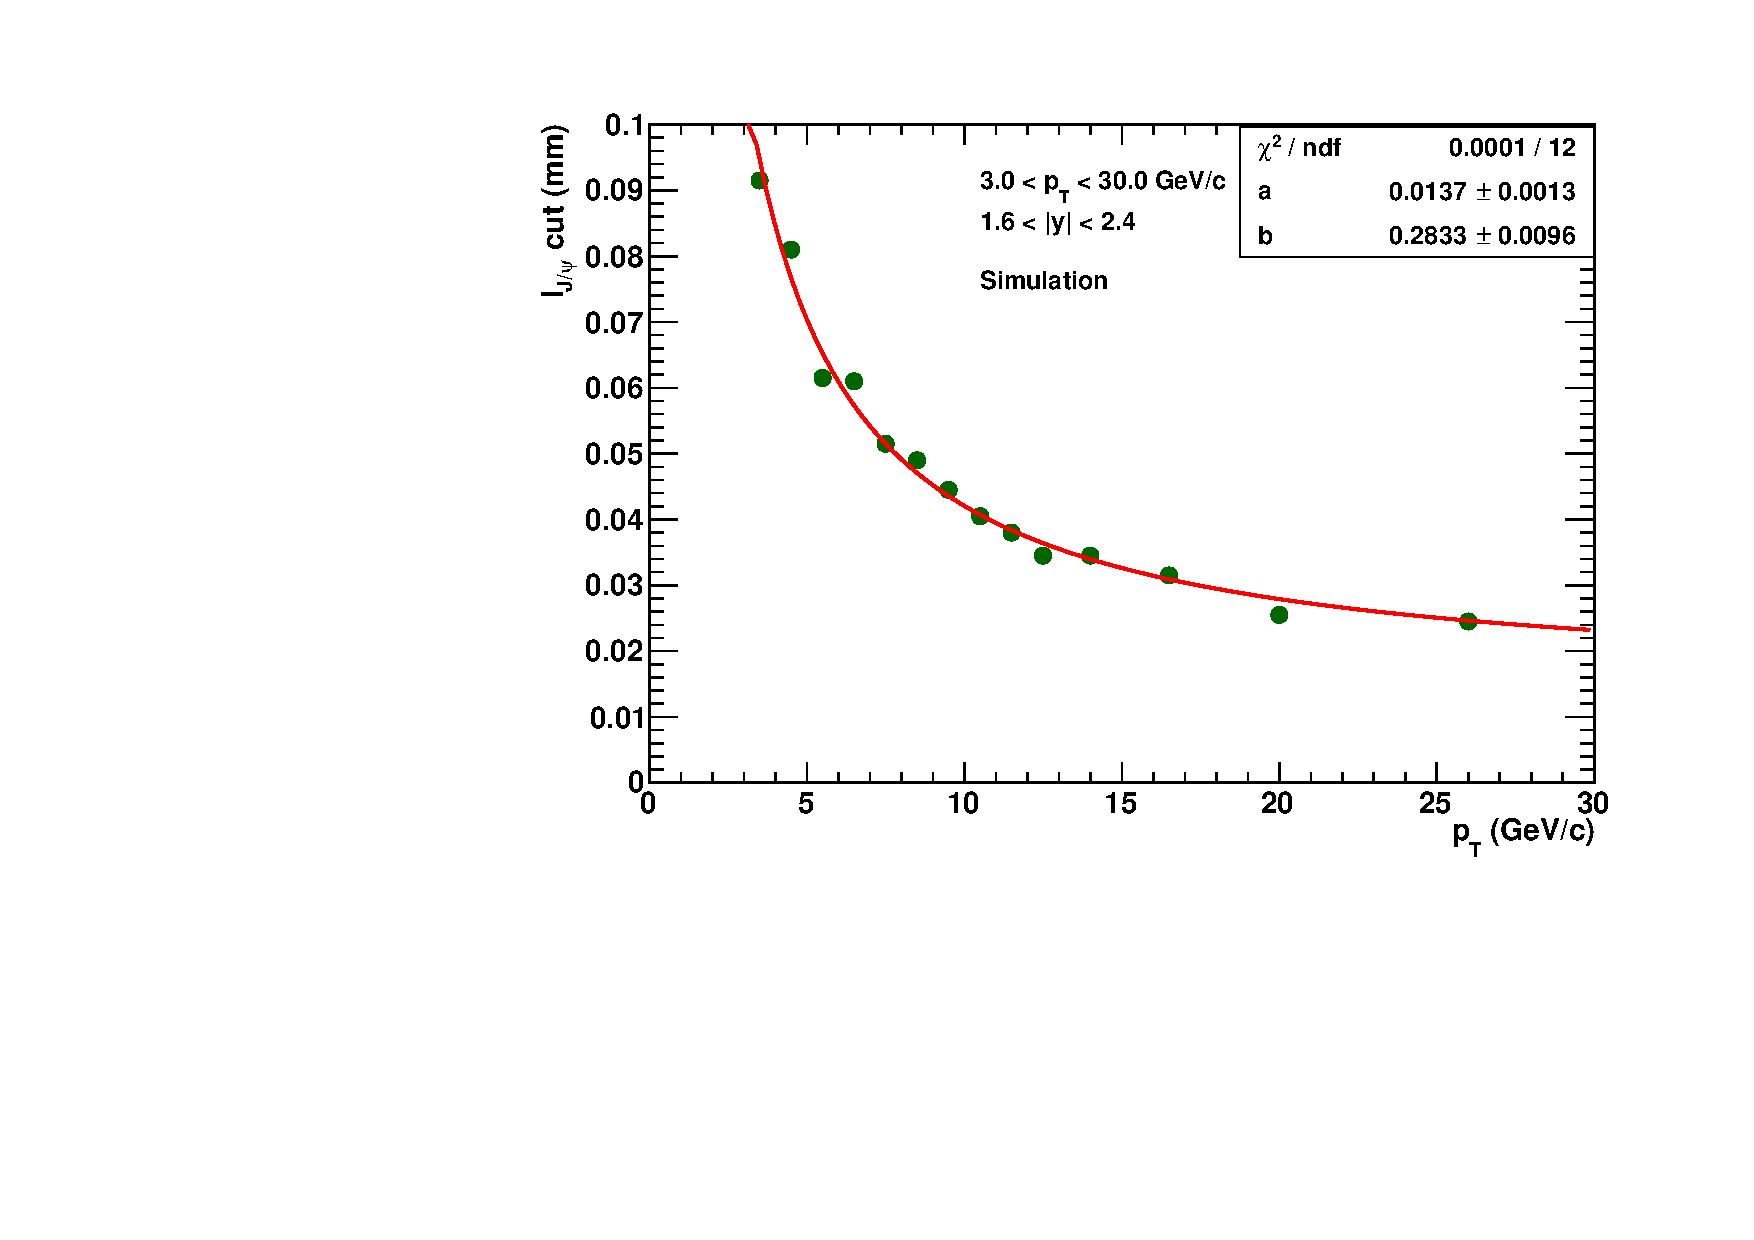
\includegraphics[width=0.48\textwidth]{Figures/Charmonia/Analysis/PsiPSignalExtraction/CtauCut/Jpsi_ppPbPbGlb_eff_0p9_Rap_1p6-2p4_Pt_3p0-30p0_Cent_0-100.pdf}
 \caption{Profile of the \ctau selection thresholds (green points) with respect to \ptMuMu, extracted from the \JPsi simulations in the mid-rapidity (left) and forward rapidity (right) regions. The fitted functions (red lines) are also displayed and the values of their parameters are shown in the box.}
 \label{fig:CtauCutPtDep}
\end{figure}

The efficiencies of passing the \ctau selection, as a function of \ptMuMu, are presented in  \fig{fig:CtauCutEff}. By construction, the \ctau selection efficiencies of prompt \JPsi mesons are close to 90\%, while it is observed to be more efficient for prompt \PsiP mesons, due to the slightly higher momentum of the muons. However, the difference between the prompt \JPsi and \PsiP efficiencies are found to be the same in \Runpp and \RunPbPb simulations. The efficiency for nonprompt \JPsi mesons, leading to a contamination from this component, is seen  to increase when going towards lower \ptMuMu values reaching up to 20\%. These efficiencies are used in \sect{sec:Charmonia_Analysis_PsiPYieldExtraction_NonPromptCorr} to subtract the nonprompt charmonium contamination from the measured ratios of \PsiP over \JPsi mesons.

\begin{figure}[htb!]
 \centering
 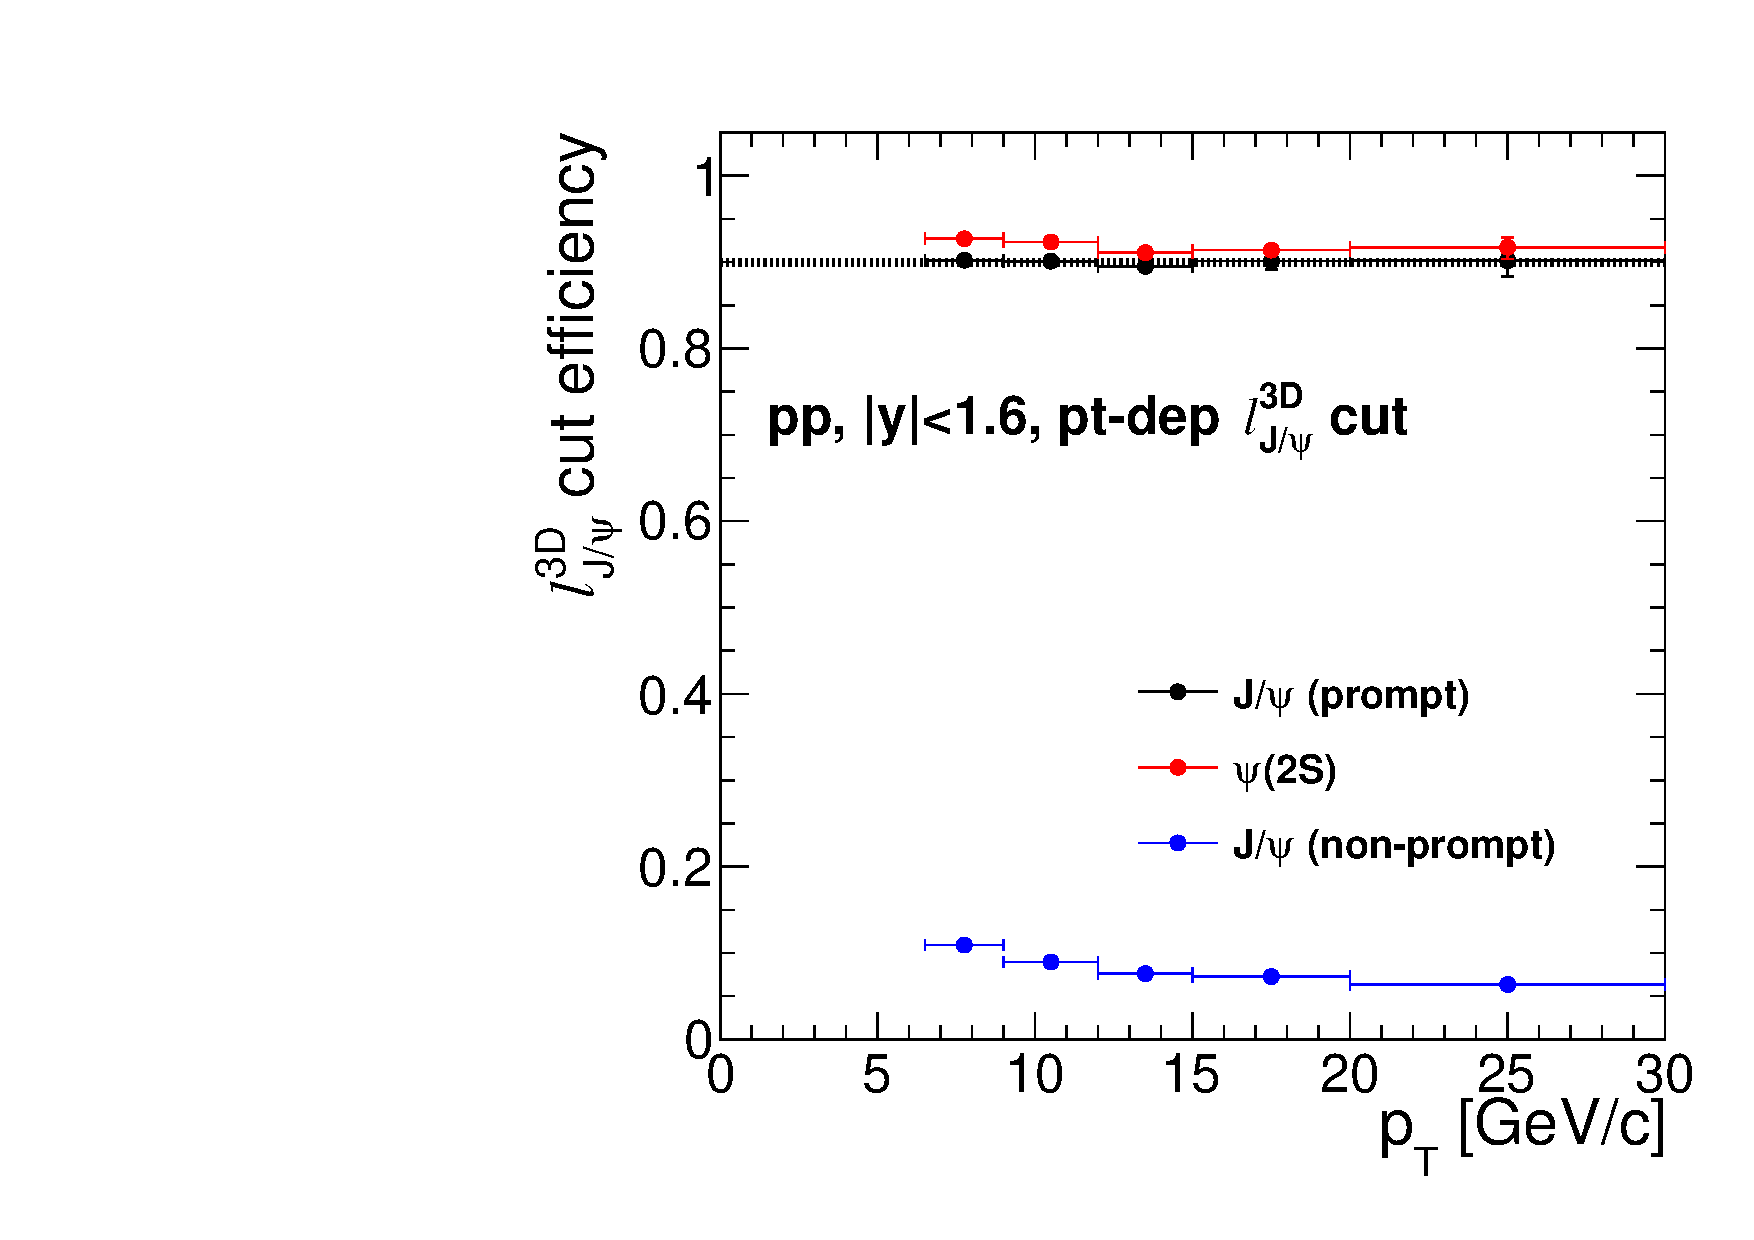
\includegraphics[width=0.45\textwidth]{Figures/Charmonia/Analysis/PsiPSignalExtraction/CtauCut/ctaucuteff_pp_pt_mid_ptdepcut.pdf}
 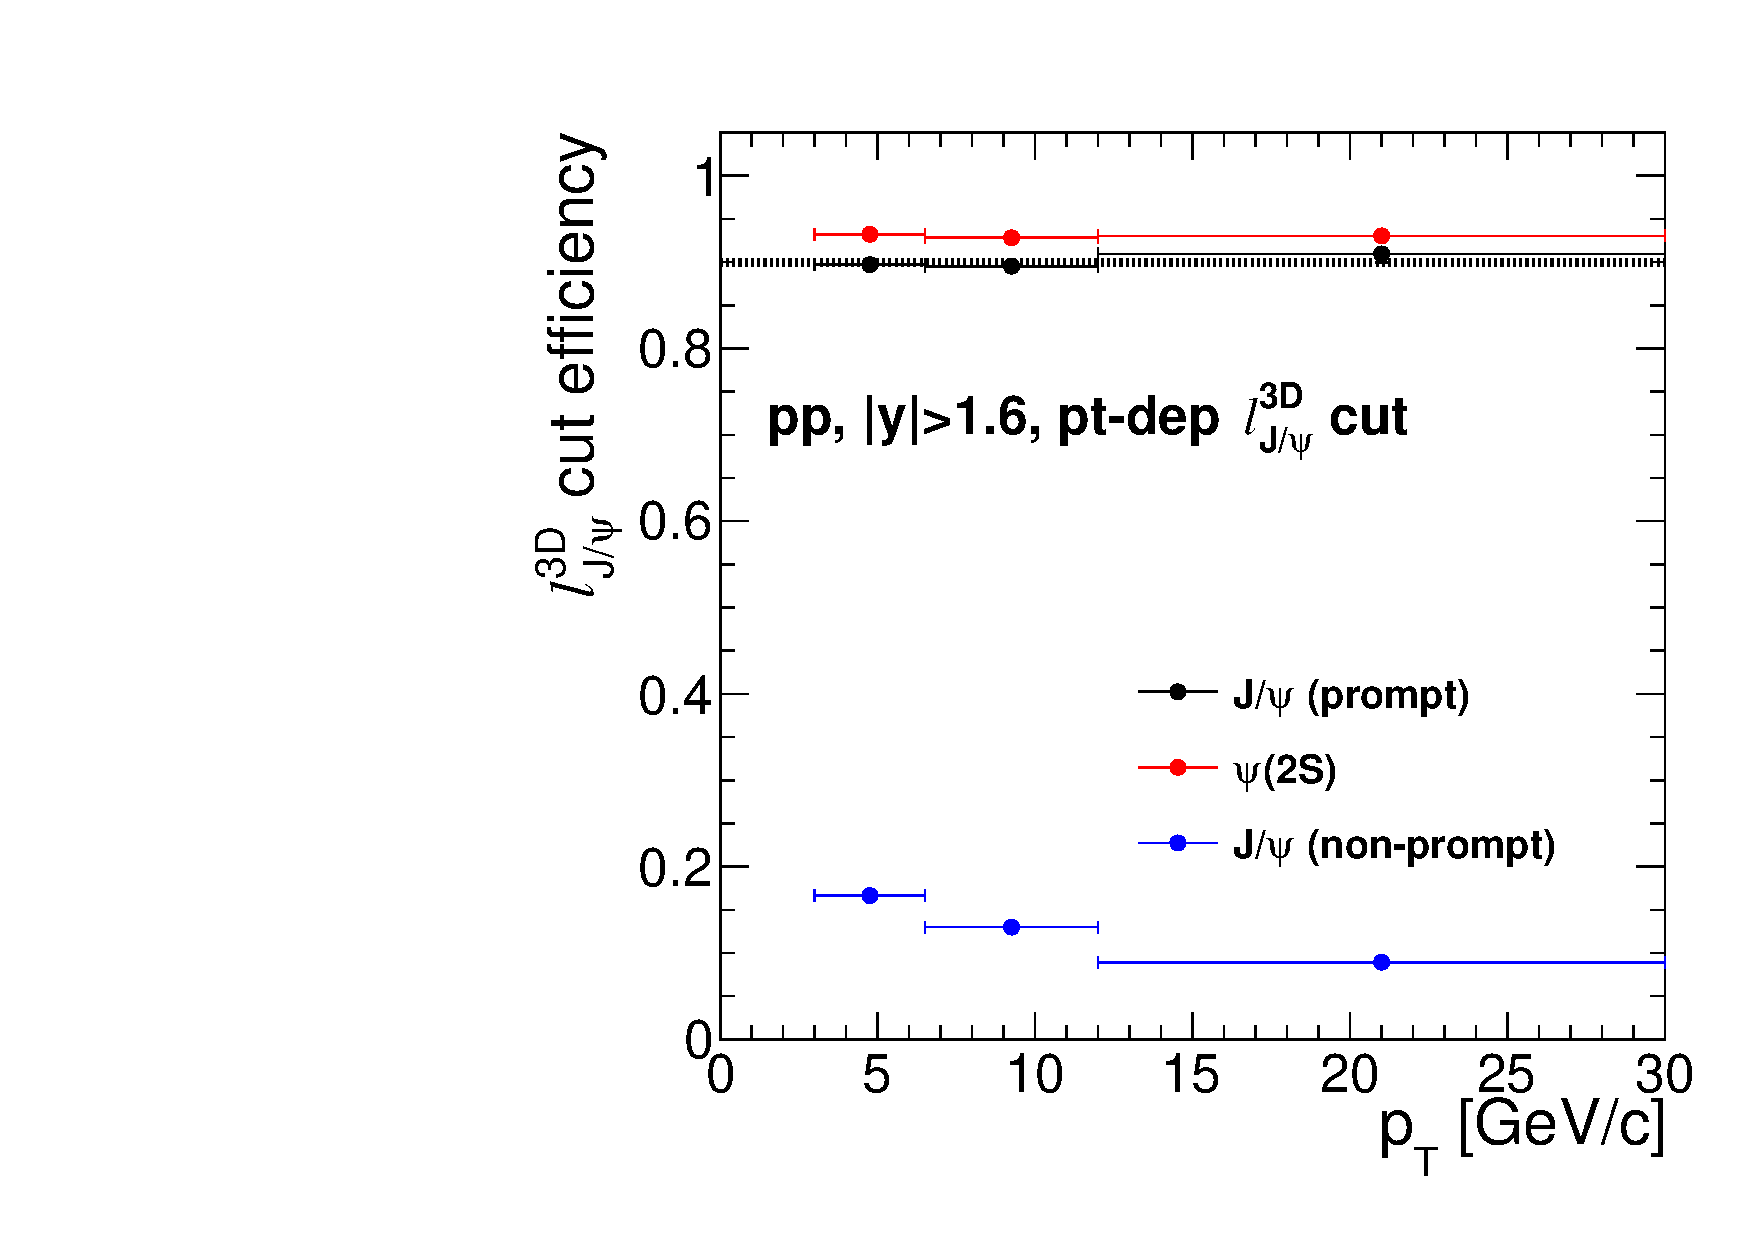
\includegraphics[width=0.45\textwidth]{Figures/Charmonia/Analysis/PsiPSignalExtraction/CtauCut/ctaucuteff_pp_pt_fwd_ptdepcut.pdf}
 \caption{Efficiency of passing the \ctau selection as a function of \ptMuMu for prompt \JPsi (black points), prompt \PsiP (red points) and nonprompt \JPsi (blue points) mesons. The results are extracted from \Runpp simulations in the mid-rapidity (left) and forward rapidity (right) regions.}
 \label{fig:CtauCutEff}
\end{figure}


\subsubsection{Fits to the dimuon invariant mass distribution}\label{sec:Charmonia_Analysis_PsiPYieldExtraction_InvMass}

The ratio of \PsiP over \JPsi meson yields is extracted separately in \Runpp and \RunPbPb collisions by performing an unbinned maximum-likelihood fit to the \mMuMu distribution within the region  $2.2 < m_{\mumu} < 4.5 ~\mathrm{GeV}/c^{2}$. The total fit model used is defined as:

\begin{equation}
 F\left(\mMuMu\right) = N_{\JPsi} \cdot \left[ M_{\JPsi}\left(\mMuMu\right) + R_{\psi} \cdot M_{\PsiP}\left(\mMuMu\right) \right] + N_{\bkg} \cdot M_{\bkg}\left(\mMuMu\right) \quad \quad
\end{equation}

where $R_{\psi}$ is the \PsiP-to-\JPsi yields ratio, $N_{\JPsi}$ ($N_{\bkg}$) is the number of \JPsi meson (background) events, and $M_{i}$ represents the \mMuMu functional form for each source of events.

The parametrisation of the signal and background \mMuMu distributions follows the same strategy used in \sect{sec:Charmonia_Analysis_JPsiYieldExtraction_InvMassPar}. The shapes of \JPsi and \PsiP mesons are described using a weighed sum of two Crystall Ball functions with common mean. Since the statistics in data is not enough to reliable fit the \PsiP mass peak, the \PsiP CB parameters are constrain to the \JPsi ones. The following criteria are used to constrain the \PsiP CB parameters when performing the data fits:
\begin{itemize}
 \item The common tail parameters are taken to be the same between the \JPsi and \PsiP CB functions ($\alpha_{\PsiP}=\alpha_{\JPsi}$, $n_{\PsiP} = n_{\JPsi}$).
 \item The weight of the \PsiP CB components is fixed to the \JPsi CB weight ($f_{\PsiP} = f_{\JPsi}$).
 \item The \PsiP CB mean parameter is fixed to the \JPsi CB mean multiplied by the mass ratio of \PsiP over \JPsi mesons ($m_{\PsiP}/m_{\JPsi} = 1.1902$)~\cite{PDG}.
 \item The two width parameters of the \PsiP CB function are fixed to the corresponding \JPsi CB widths scaled by the \PsiP to \JPsi mass ratio ($\sigma^{\PsiP}_{\text{CB},i} = (m_{\PsiP}/m_{\JPsi})\cdot\sigma^{\JPsi}_{\text{CB},i}$).
\end{itemize}

The \JPsi CB parameters are tuned using the prompt \JPsi simulations after applying the \ctau selection defined in the previous section. The parameter values extracted from the \Runpp and \RunPbPb simulations are found to be in good agreement, and thus, the results obtained from the \Runpp simulation are used. The nominal values of the CB parameters are presented in \tab{tab:MCSignalShapeParam_PsiP}, where those that appear in bold are fixed when performing the fits to \mMuMu distribution in data. The parameters that are left free in the data fits are: the weight of the CB components $f_{\JPsi}$, the mean parameter $m_{\JPsi}$, the width parameter $\sigma^{\JPsi}_{\text{CB},1}$, the number of \JPsi mesons $N_{\JPsi}$, and the ratio of \PsiP over \JPsi meson yields $R_{\psi}$. When fitting the \Runpp data, the width parameter $\sigma_{\text{CB}, 2}$ is also left free. 

\begin{table}[htb!]
  \centering
  \smallskip
  \begin{tabular}{llccccc}
    \hline\hline
    \rapMuMu & \ptMuMu [\GeVc] & \fJPsi & \aJPsi & \nnJPsi & ${\sigma_{\CB,2}/\sigma_{\CB,1}}$ \\
    \hline
    0--1.6   & 6.5--30.0 & 0.71 & \textbf{1.87} & \textbf{1.76} & 1.94 \\
    1.6--2.4 & 3.0--30.0 & 0.82 & \textbf{2.18} & \textbf{1.46} & 1.79
  \end{tabular}
  \caption{Parameters extracted for the double Crystal Ball function from the prompt \JPsi-meson \Runpp simulation after applying the \ctau selection. The values shown correspond to the \pt-centrality integrated fits. The CB parameters fixed to simulation when performing the data fits are shown in bold font.}
  \label{tab:MCSignalShapeParam_PsiP}
\end{table}

In the case of the background, the \mMuMu shape is modelled using a Chebyshev function of order $N$, where the order for each analysis bin is defined using a LLR test as performed in \sect{sec:Charmonia_Analysis_JPsiYieldExtraction_InvMassPar}. The selected background Chebyshev functions are of first or second order.

The results of the fits to the \mMuMu distribution in \RunPbPb and \Runpp collisions, performed in the \pt-centrality-inclusive region at mid-rapidity after applying the \ctau selection, are shown in \fig{fig:MassPsiP}.

\begin{figure}[htb!]
 \centering
 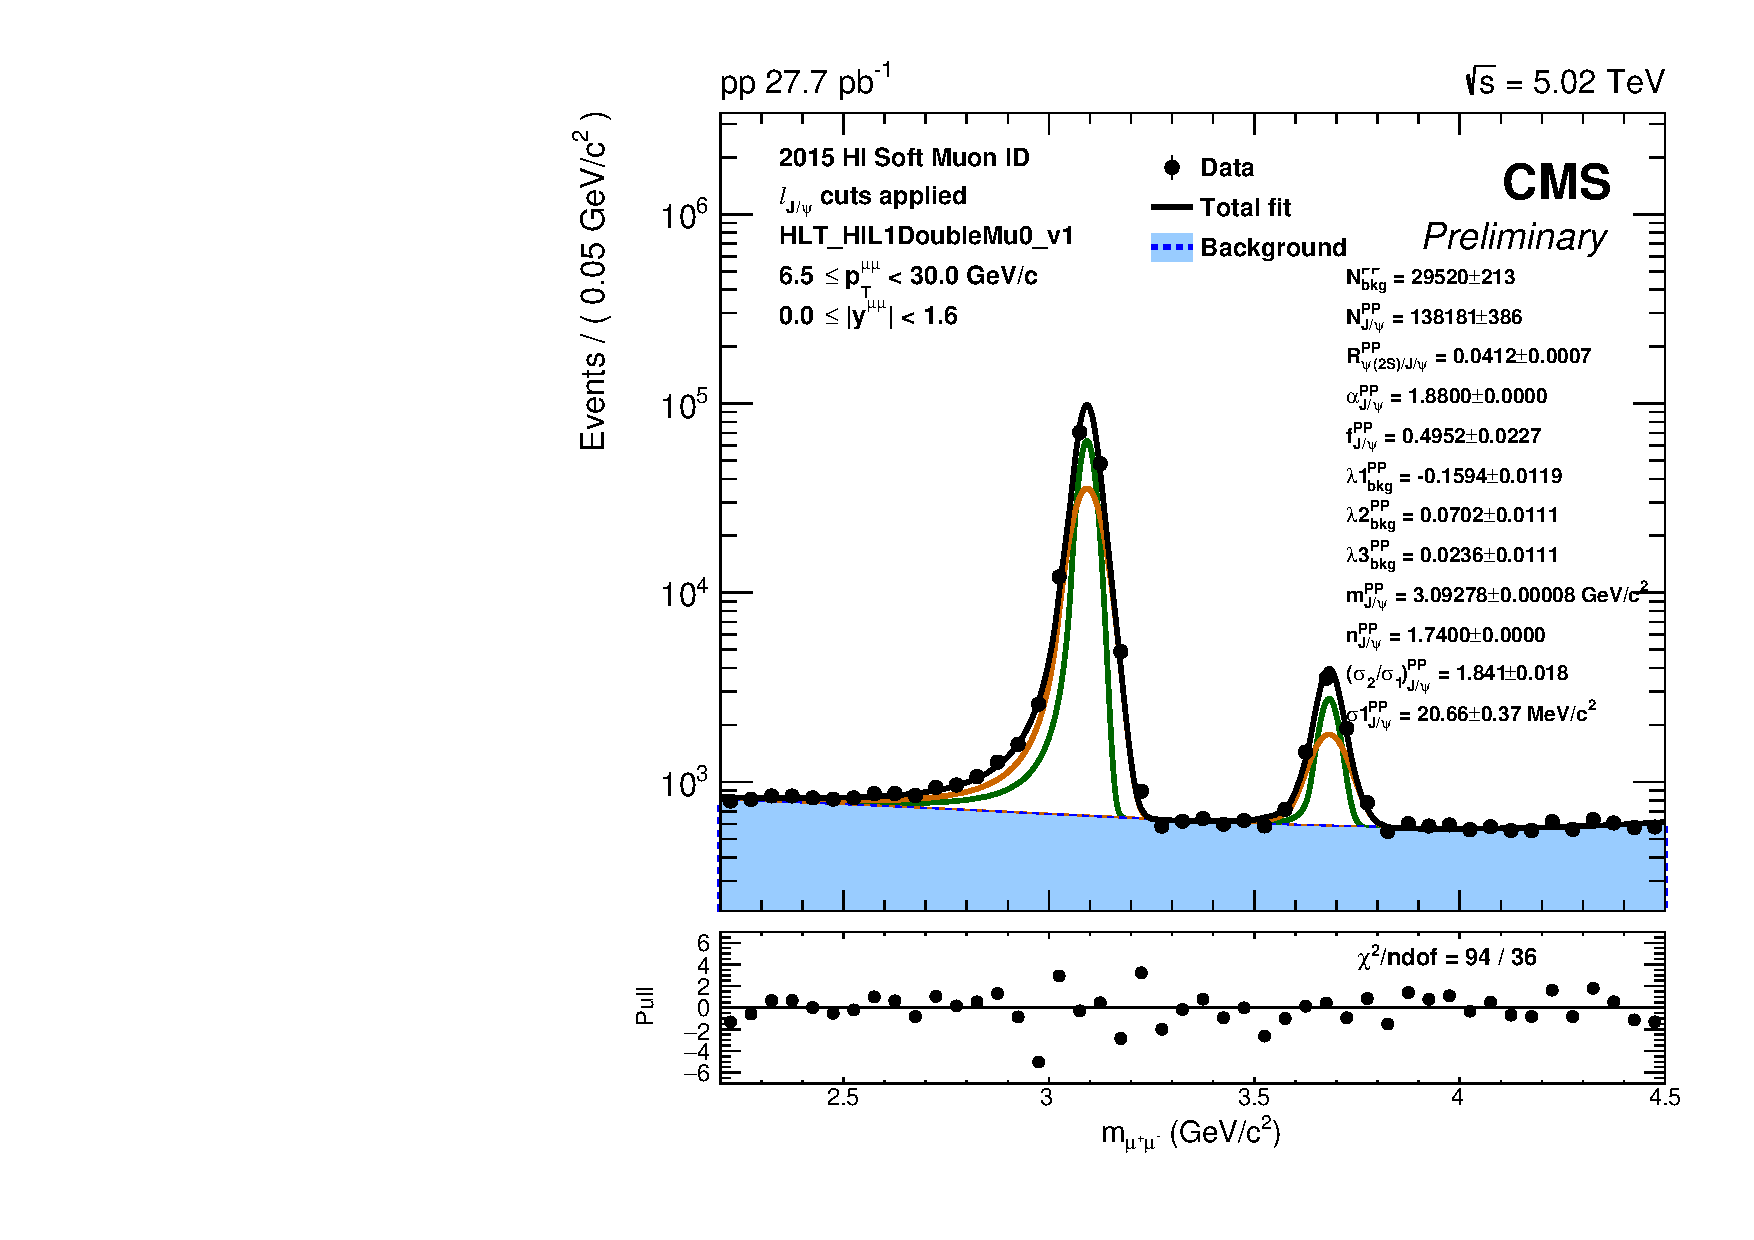
\includegraphics[width=0.45\textwidth]{Figures/Charmonia/Analysis/PsiPSignalExtraction/mass/DATA_Psi2SJpsi_PP_Jpsi_DoubleCrystalBall_Psi2S_DoubleCrystalBall_pt65300_rap016_cent0200.pdf}
 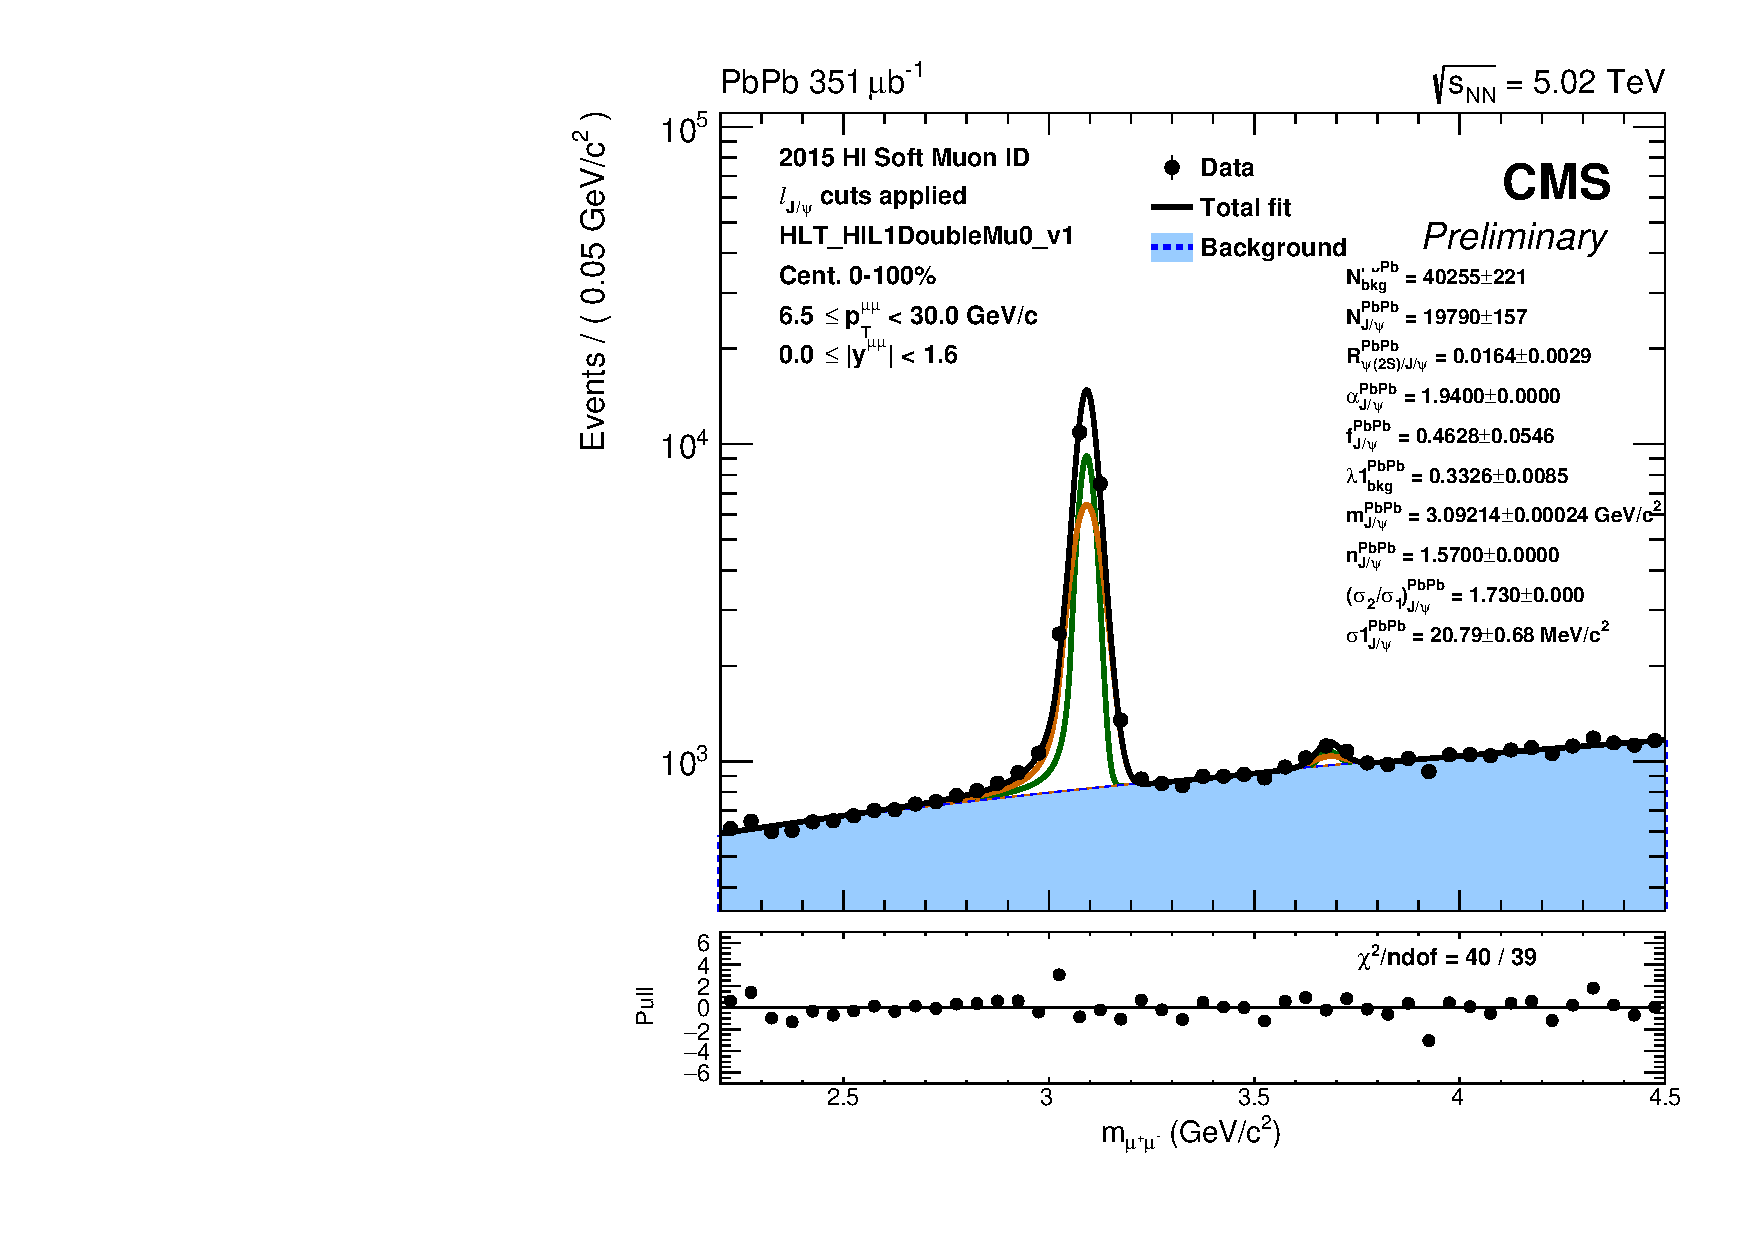
\includegraphics[width=0.45\textwidth]{Figures/Charmonia/Analysis/PsiPSignalExtraction/mass/DATA_Psi2SJpsi_PbPb_Jpsi_DoubleCrystalBall_Psi2S_DoubleCrystalBall_pt65300_rap016_cent0200.pdf}
\caption{Fits to the \mMuMu distribution in \Runpp (left) and \RunPbPb (right) collisions. The results correspond to dimuon events derived in \pt-centrality-inclusive region at mid-rapidity after applying the \ctau selection. The black line represents the total fit model while the blue filled area represents the fitted background shape.}
 \label{fig:MassPsiP}
\end{figure}


\subsubsection{Correction for nonprompt charmonium contamination}\label{sec:Charmonia_Analysis_PsiPYieldExtraction_NonPromptCorr}

Since the main goal of the analysis is to measure the ratio of prompt \PsiP over \JPsi meson yields, it is important to correct for the amount of nonprompt charmonia that remains after selecting dimuons with low \ctau, even though they represent a small fraction of the sample. In order to do this, four categories of events are considered as illustrated in \fig{fig:abcd}, which are:

\begin{itemize}
 \item (A): Prompt charmonia passing the \ctau selection.
 \item (B): Nonprompt charmonia passing the \ctau selection.
 \item (C): Prompt charmonia failing the \ctau selection.
 \item (D): Nonprompt charmonia failing the \ctau selection.
\end{itemize}

\begin{figure}[htb!]
 \centering
 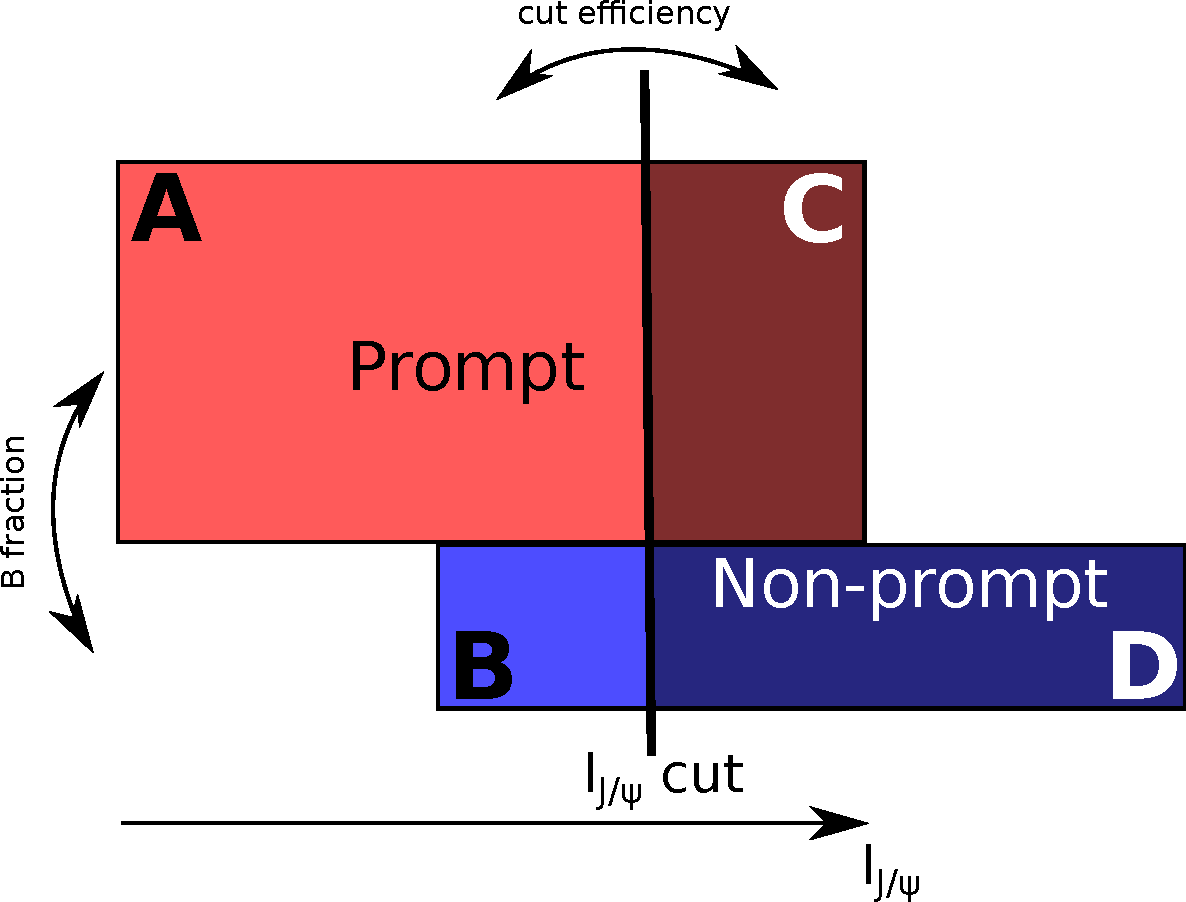
\includegraphics[width=0.5\textwidth]{Figures/Charmonia/Analysis/PsiPSignalExtraction/NonPromptCorr/abcd.pdf}
 \caption{Definition of the different categories of events considered for the subtraction of nonprompt charmonia.}
 \label{fig:abcd}
\end{figure}

Based on the categories presented in \fig{fig:abcd}, the objective is to extract the number of \textit{prompt} $\psi$ (\PsiP or \JPsi) mesons defined in the region $A + C$. The number of charmonia in the region $A + B$ (labelled as \textit{pass}) is extracted from the \mMuMu fits after selecting dimuons passing the \ctau selection. Furthermore, the charmonium yields in the region $C + D$ (referred as \textit{fail}) are simply measured by inverting the \ctau selection (i.e. selecting dimuons with high \ctau) and redoing the fits to the \mMuMu spectrum following the same procedure used in the previous section.

Using the \ctau selection efficiencies estimated from the prompt ($\epsilon^{\text{P}}_{\psi}$) and nonprompt ($\epsilon^{\text{NP}}_{\psi}$) charmonium simulations, and the charmonium yields extracted from the \mMuMu fits after applying the \ctau selection ($N^{\text{pass}}_{\psi}$) and inverting it ($N^{\text{fail}}_{\psi}$), one can derived the following equation:

\begin{equation}
  N^{\text{pass}}_{\psi} = \left[ \epsilon^{\text{P}}_{\psi} \cdot f^{\text{P}}_{\psi} + \epsilon^{\text{NP}}_{\psi} \cdot \left(1-f^{\text{P}}_{\psi}\right) \right] \cdot N^{\text{tot}}_{\psi}
 \label{eq:PassPsiP}
\end{equation}

where $f^{\text{P}}_{\psi}$ is the fraction of prompt charmonia and $N^{\text{tot}}_{\psi}$ is the total amount of $\psi$ mesons (i.e. $N^{\text{tot}}_{\psi} = N^{\text{pass}}_{\psi} +   N^{\text{fail}}_{\psi}$). One can then deduce from \eq{eq:PassPsiP} the number of prompt charmonia, given by:

\begin{equation}
 N^{\text{P}}_{\psi} = f^{\text{P}}_{\psi} \cdot N^{\text{tot}}_{\psi} = \frac{N^{\text{pass}}_{\psi} - \epsilon^{\text{NP}}_{\psi}\cdot{N^{\text{tot}}_{\psi}}}{\epsilon^{\text{P}}_{\psi} - \epsilon^{\text{NP}}_{\psi}}
 \label{eq:passprompt}
\end{equation}

The ratios of prompt \PsiP over \JPsi meson yields are then determined for \Runpp and \RunPbPb collisions, according to:

\begin{equation}
 R^{\text{P}}_{\psi} = \frac{N^{\text{P}}_{\PsiP}}{N^{\text{P}}_{\JPsi}}
 \label{eq:DRPrompt}
\end{equation}

The largest relative difference between the ratios of charmonium yields extracted from the \mMuMu distribution of dimuons passing the \ctau selection ($R^{\text{pass}}_{\psi}$) and the ratios of prompt charmonium yields ($R^{\text{P}}_{\psi}$), is found to be 6\% for \Runpp data and 18\% for \RunPbPb data. Regarding the double ratio, the largest relative difference is 16\%.

% END OF SUBSECTION